\documentclass[12pt]{article}
\usepackage[a4paper,hmargin=1.5cm,top=2cm,bottom=2.5cm]{geometry}
\usepackage{fontspec}
\usepackage{xeCJK}
\usepackage[shortlabels,inline]{enumitem}
\usepackage{amsmath}
\usepackage{amssymb}
\usepackage{caption}
\usepackage{chemformula}
\usepackage{siunitx}
\usepackage{tikz}
\usepackage{xeCJKfntef}
\usepackage{pgfplots}
\usepackage{lastpage}
\usepackage{fancyhdr}
\pagestyle{fancy}
\renewcommand{\headrulewidth}{0pt}
\fancyhead{}
\cfoot{\thepage\ /\ \pageref{LastPage}}
\setlength{\parindent}{0pt}
\setCJKmainfont{Noto Serif CJK TC}
\linespread{1.15}

\begin{document}
{
  \Large \bfseries 練習題 \hfill 2023/07/05
}
\begin{enumerate}[left=0pt]
  \item 已知乙烷(\ch{C2H6})和丙醇(\ch{C3H7OH})在燃燒時,皆會生成二氧化碳與水蒸氣,其反應式如下:
  \begin{align*}
    \textrm{乙烷} + \textrm{氧氣} &\longrightarrow \textrm{二氧化碳} + \textrm{水} \tag*{反應(一)} \\
    \textrm{丙醇} + \textrm{氧氣} &\longrightarrow \textrm{二氧化碳} + \textrm{水} \tag*{反應(二)}
  \end{align*}
  試回答以下問題。(\ch{H}、\ch{C}、\ch{O} 的原子量分別為 $1$、$12$、$16$)
  \begin{enumerate}[left=0pt,label=(\arabic*)]
    \item 將反應(一)與反應(二)當中的中文名稱\CJKunderdblline{改寫為化學式},並\CJKunderdblline{加上係數}以平衡反應式。\vspace{30ex}
    \item 計算乙烷、丙醇與二氧化碳的分子量。\vspace{30ex}
    \item 當等質量的乙烷與丙醇完全燃燒時,所生成的二氧化碳質量比為何?
  \end{enumerate}
  \newpage
  \item 將一顆球自地面鉛直上拋,球上升一段高度後會向下墜落,最終落至地面。已知開始上拋時球的速度大小為 \qty{20}{m/s},且重力加速度為 \qty{10}{m/s^2},試回答以下問題。(須附上各物理量的單位)
  \begin{enumerate}[left=0pt,label=(\arabic*)]
    \item 繪製物體由開始上拋至落地期間,其速度 $v$ 與時間 $t$ 的關係圖。(以鉛直向上為正向)
    \begin{center}
      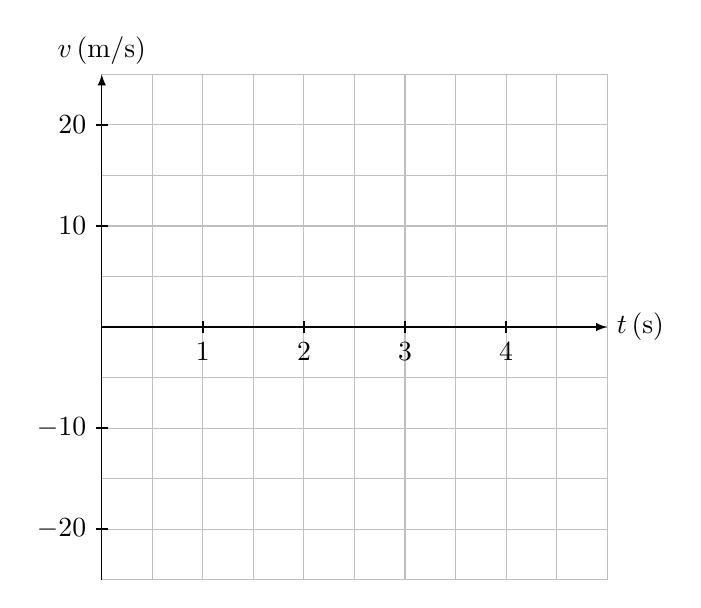
\begin{tikzpicture}
        \begin{axis}[
          height=8cm,width=8cm,axis lines=center,axis line style={-latex},
          xlabel={$t$\,(\unit{s})},
          ylabel={$v$\,(\unit{m/s})},
          xmin=0,xmax=5,ymin=-25,ymax=25,
          grid=both,
          xtick={0,1,...,4},minor xtick={0,.5,...,5},
          ytick={-20,-10,...,20},minor ytick={-25,-20,-15,...,25},
          every x tick/.style={black,thick},every y tick/.style={black,thick},
          minor tick style={draw=none},
          xlabel style={at={(axis description cs:1,.5)},anchor=west},
          ylabel style={at={(axis description cs:0,1)},align=center,anchor=south}
        ]
        \end{axis}
      \end{tikzpicture}
    \end{center}
    \item 計算物體所能抵達的最大高度。\vspace{35ex}
    \item 計算物體自開始上拋至落地期間的\CJKunderdblline{平均速率}。
  \end{enumerate}
\end{enumerate}
\end{document}
